
% LaTeX Beamer Slide Presentation Template

\documentclass{beamer}

%% FORMATTING
% ----------------------------------------------------------------------------- %
%\usepackage[margin=1in]{geometry} % margins
%\usepackage[doublespacing]{setspace} % line spacing
\usepackage{
    multicol, % multiple columns
    blindtext, % \blindtext (lorem ipsum)
    lipsum,
}
\usepackage{parskip} % distance between paragraphs; care with theorem environment
\setlength{\parskip}{0.5cm plus4mm minus3mm}
\usetheme{Madrid}
\graphicspath{{figures/}} % graphics should go into the ./figures/ folder
\blindmathtrue


%% MATH %%
% ----------------------------------------------------------------------------- %
\usepackage{ 
    mathtools, % advanced math (superset of amsmath)
    % thmtools,
    amssymb, % additional math symbols
    amsthm, % proof environment and \theoremstyle
    mathrsfs, % scripty math
    % stmaryrd % contains \lightning
}

%% OPERATORS / DELIMITERS
% ----------------------------------------------------------------------------- %
% \operatorname{Example} for single use
% \DeclareMathOperator{\example}{Example}
\DeclarePairedDelimiter{\abs}{\lvert}{\rvert}
\DeclareMathOperator{\injects}{\hookrightarrow}
\DeclareMathOperator{\iso}{\cong}
\DeclareMathOperator{\Aut}{Aut}
\DeclareMathOperator{\Orb}{Orb}

%% REFERENCE
% ----------------------------------------------------------------------------- %
\usepackage{ 
    % nameref, % \nameref
    % hyperref % hyperlink/reference
}



\title{Happy Ending Extensions via SAT Solvers}
\author{Daniel Taylor, Julia Rima, Sumanth Ravipati
\\ with Dr. Walter Morris}
\institute{George Mason University, MEGL}
\date{\today}

%% template for frames:

%\section{} % shown in Table of Contents
%\subsection{} % shown in Table of Contents
%\begin{frame} 
%    \frametitle{} % shown at top of slide
%        % some content
%\end{frame}

\begin{document}

%% title page
% ----------------------------------------------------------------------------- %
\begin{frame}
    \titlepage
\end{frame}

%% table of contents
% ----------------------------------------------------------------------------- %
\begin{frame}
    \frametitle{Table of Contents}
        \tableofcontents
\end{frame}

%% content slides

% ----------------------------------------------------------------------------- %

\section{Review}

\begin{frame}
    \frametitle{Review}
    \begin{itemize}
        \item Esther-Klein
        \item General n-gons
        \item SAT Solvers
    \end{itemize}
\end{frame}

% ----------------------------------------------------------------------------- %
\section{Extension to 3D Space}

\subsection{3-Polytopes} 
\begin{frame}
    \frametitle{3-Polytope Considerations}
    \begin{itemize}
        \item General position w.r.t. 3D space
        \item Categories of 3-polytopes
        \item Searching for specific polytopes
    \end{itemize}
\end{frame}

% ----------------------------------------------------------------------------- %

\begin{frame}
\frametitle{Tetrahedron}
    \begin{figure}[h] % figure specifier [h] for here (in the slide)
        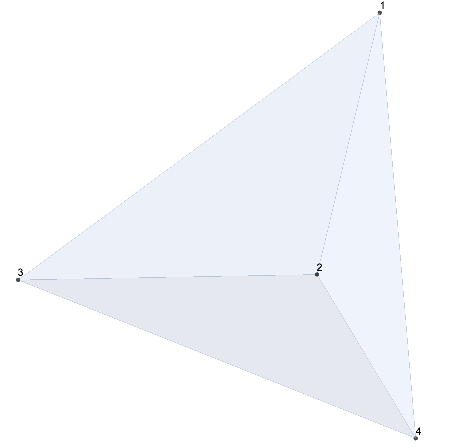
\includegraphics[scale = 0.4]{Tetra.png} % name of graphic in the folder 'figures' at the same level as the .tex source
        \caption{Tetrahedron}
    \end{figure}
\end{frame}

% ----------------------------------------------------------------------------- %

\begin{frame}
\frametitle{Triangular Bipyramid}
    \begin{figure}[h] % figure specifier [h] for here (in the slide)
        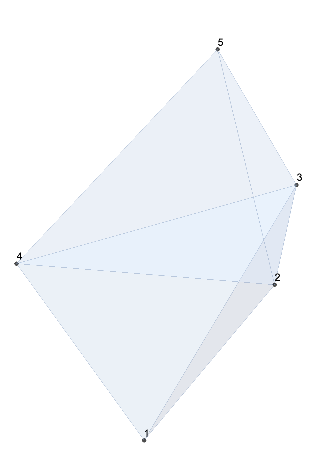
\includegraphics[scale = 0.4]{TriBiPy.png} % name of graphic in the folder 'figures' at the same level as the .tex source
        \caption{Triangular Bipyramid in General Position}
    \end{figure}
\end{frame}

% ----------------------------------------------------------------------------- %

\begin{frame}
\frametitle{Octahedron}
    \begin{figure}[h] % figure specifier [h] for here (in the slide)
        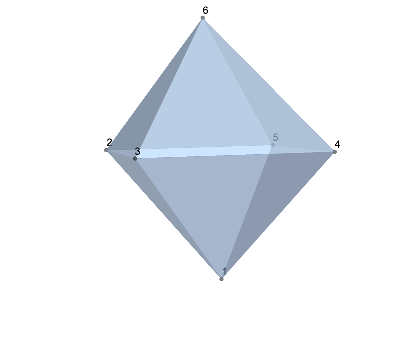
\includegraphics[scale = 0.4]{Octo.png} % name of graphic in the folder 'figures' at the same level as the .tex source
        \caption{Octahedron in General Position}
    \end{figure}
\end{frame}

% ----------------------------------------------------------------------------- %

\begin{frame}
\frametitle{Cyclic Polytope}
    \begin{figure}[h] % figure specifier [h] for here (in the slide)
        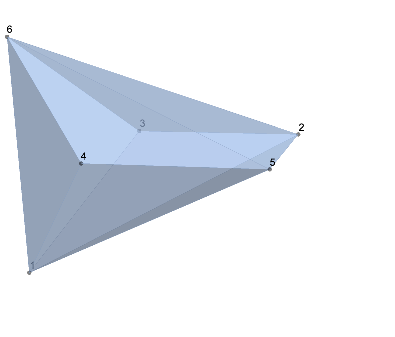
\includegraphics[scale = 0.4]{Cyclic.png} % name of graphic in the folder 'figures' at the same level as the .tex source
        \caption{Cyclic Polytope in General Position}
    \end{figure}
\end{frame}

% ----------------------------------------------------------------------------- %

\subsection{Constraints}
\begin{frame}
    \frametitle{Constraints}
    \begin{itemize}
        \item Convexity
        \item Acyclicity
        \item Form desired polytope
        \item Degree(s) of freedom
        \item Listing out chirotopes
    \end{itemize}
\end{frame}
   
% ----------------------------------------------------------------------------- %

\section{Next Steps}

\begin{frame}
    \frametitle{Next Steps}
    \begin{itemize}
        \item More vertices
        \item Higher dimensions
        \item Specific polytopes
        \item Searching for general formulas
        \item General SAT solvers
    \end{itemize}
\end{frame}
   
% ----------------------------------------------------------------------------- %
    
\end{document}